\begin{center}
    \textbf{--------- Lezione 7 - 25 marzo 2021 ---------}
\end{center}

\section{Panoramica}
Le due librerie principali per lo sviluppo di applicazioni AR sono:
\begin{itemize}
    \item ARKit di Apple: è utilizzabile sui device mobili Apple recenti e non utilizzabile su simulatore
    \item ARCore di Google: può essere utilizzata in nativo su Android ed è utilizzabile, con alcune limitazioni, su simulatore
\end{itemize}
\subsection{Macro funzionalità}
Per realizzare applicazioni in realtà aumentata, ARKit e ARCore forniscono funzionalità per semplificare le seguenti operazioni:
\begin{itemize}
    \item Registration e Tracking
    \item Scene
    \item Display
    \item Interaction
\end{itemize}

ARKit e ARCore condividono alcuni concetti base:
\begin{itemize}
    \item scene (ARKit) / session (ARCore): due nomi diversi per lo stesso concetto, che rappresenta l'ambiente rispetto al quale effettuiamo la registration. Gli oggetti virtuali e reali sono posizionati nel sistema di riferimento della scena/sessione. Fornisce le chiamate per accedere agli altri elementi di AR
    \item configuration: definisce le caratteristiche della scena / sessione da creare:
    \begin{itemize}
        \item rispetto a cosa facciamo la registration, ad esempio rispetto all'ambiente 3D circostante, viene creato un sistema di riferimento in una posizione iniziale e si tiene traccia dello spostamento rispetto a questo sistema
        \item rispetto a cosa siamo interessati a riconoscere
    \end{itemize}
    \item ancore: rappresentano dei punti di riferimento agli oggetti virtuali o reali identificati. Es: quando un oggetto viene riconosciuto, viene associato ad un’ancora. Attraverso l’ancora possiamo risalire alla posizione e rotazione (6DOF) dell'oggetto rispetto alla scena. Le ancore si usano ad esempio quando riconosciamo i piani ed ogni piano è rappresentato dalla propria ancora
    \item hitTest/rayCasting: si tratta di un’operazione per convertire le coordinate schermo (2D) in un punto 3D. Concettualmente devo considerare il raggio, che “esce” dal device verso lo spazio, che interseca zero o più oggetti (reali o virtuali) ed hitTest ritorna l’insieme di questi oggetti
\end{itemize} 

\subsection{Comprendere la scena}
ARKit e ARCore forniscono alcuni strumenti che semplificano il processo di comprensione della scena:
\begin{itemize}
    \item riconoscimento piani
    \item riconoscimento immagini (2D): la procedura avviene in 3 passi:
        \begin{itemize}
            \item aggiunta dell'immagine alle risorse del progetto: si fornisce ad ARKit/ARCore l'immagine da riconoscere e la dimensione attesa nel mondo reale
            \item modifica della configurazione della scena, indicando, da codice, che si vuole riconoscere quell'immagine
            \item specificare cosa fare quando l'immagine viene riconosciuta: si gestisce l'evento di quando l'ancora relativa a quell'immagine viene aggiunta
        \end{itemize}
    \item riconoscimento dei volti
    \item riconoscimento oggetti (3D): dobbiamo prima ottenere un modello 3D dell'oggetto e poi il procedimento di riconoscimento è analogo a quanto avviene per le immagini 2D 
\end{itemize}

\section{Alcune funzionalità di ARKit 4}
\subsection{AR multiuser}
Sia in ARKit che in ARCore si possono avere più scene/sessioni condivise tra più utenti. 
Prendiamo ad esempio un utente identifica dei feature point e poi si identifica tramite l'ambiente. Se quelle stesse informazioni vengono condivise con un altro utente e il device di questo, riesce a capire dove si trova rispetto ai fp del primo utente, possiamo fare la registrazione rispetto ad un sistema di riferimento comune. Questo permette di mostrare un oggetto virtuale nello stesso punto a diversi utenti con diverse angolazioni. 
\begin{center}
    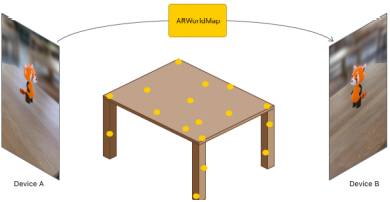
\includegraphics[width=.7\textwidth]{images/MobiDEV/5. augmented reality in pratica/ar multiuser.PNG}
\end{center}

\subsection{Scene geometry}
I device che hanno un sensore di profondità (Lidar) possono creare una ricostruzione topologica dell'ambiente. La libreria AR per i dispositivi con Lidar mette a disposizione funzionalità per:
\begin{itemize}
    \item riconoscere gli oggetti
    \item calcolare quando un oggetto si interpone tra la camera e un oggetto virtuale, così da risolvere il problema dell'occlusione
    \item permettere agli oggetti virtuali di rispettare alcune regole della fisica nell'interazione con oggetti del mondo reale (ad esempio due oggetti che non si possono compenetrare)
\end{itemize} 
Attraverso il lidar è anche possibile andare a creare una configurazione chiamata body tracking dove il sistema riconosce le principali articolazioni del corpo e ce le restituisce come nodi, ovvero punti che possiamo tracciare, cosicché possiamo calcolare la posizione del corpo e come si muove l'utente. Questa procedura si chiama \textbf{Motion capture}.